\documentclass[11pt]{article}

\usepackage{../algebra}

\begin{document}

\coverpage{2}

% hw problem 1 -----------------------------------------------------------------

\begin{exercise}{47}{9}
    \problem{
        If $G$ is a group in which $a^2 = e$ for all $a \in G$, show that $G$ is abelian.
    }
    \proof{
        First note that $a^2 = e$ for all $a \in G$ implies that for every $a \in G$ $a^{-1} = a$ (for $a^{-1}$ is the element that satisifes $aa^{-1} = e$).
        Now pick any $x,y \in G$.
        Since $G$ is a group, we have $(xy)(xy)^{-1} = e$ and $(xy)^{-1} = y^{-1}x^{-1}$.
        Our assumption that $a^2 = e$ for all $a \in G$ allows us to say that $y^{-1}x^{-1} = yx$.
        Additionally, that same assumption tells us that $(xy)^{-1} = xy$.
        This gives the chain of equalities
        $$ xy = (xy)^{-1} = y^{-1}x^{-1} = yx $$
        Since $x,y$ were arbitrary members of $G$, we have just shown that $G$ is abelian.
    }
\end{exercise}

% hw problem 2 -----------------------------------------------------------------

\begin{exercise}{47}{18}
    \problem{
        If $G$ is a finite group of even order, show that there must be an element $a \neq e$ such that $a = a^{-1}$.
    }
    \proof{
        Suppose not, that is, suppose we have a finite group $G$ of even order such that $a = e$ is the only element to satisfy $a = a^{-1}$ for any $a \in G$.
        Let's define a map $f: G \to G$ which takes $x \in G$ to $x^{-1} = y \in G$.
        The map $f$ is well defined because each element in a group has an inverse.
        Note that $f$ must be a bijection ($f$ is 1-1 because inverses are unique in a group and $f$ is onto because each element in a group is an inverse).
        Further, $ff(x) = f(f(x)) = x$ because $f(x)x = yx = e$. \parspace
        Since $ff(x) = x$ for all $x \in G$, every element in $G$ is part of a 2-cycle or a 1-cycle under $f$.
        We assumed that $e$ is the only element to be its own inverse, which is equivalent to saying $e = f(e)$ is the only 1-cycle.
        Therefore, the remaining $|G|-1$ elements must be part of 2-cycles.
        But $|G|-1$ is odd so it cannot be broken into disjoint pairs.
        So we have reached a contradiction and it must be the case that some $a \in G$ ($a \neq e$) satisfies $a = a^{-1}$.
    }
\end{exercise}

% hw problem 3 -----------------------------------------------------------------

\begin{exercise}{47}{24}
    \problem{
        If $G$ is the dihedral group of order $2n$ as defined in Example 10, prove that
        \begin{enumerate}[label=(\alph*)]
            \item If $n$ is odd and $a \in G$ is such that $a b = ba$ for all $b \in G$, then $a = e$.
            \item If $n$ is even, show that there is an $a \in G$, $a \neq e$, such that $a b = b  a$ for all $b \in G$.
            \item If $n$ is even, find all the elements $a \in G$ such that $a  b = b  a$ for all $b \in G$.
        \end{enumerate}
    }
    \proof{
        Before going in to each section, we prove some facts about any dihedral group.
        First, we note that $f^{-1} = f$ and $(r^{-1})^j = r^{n-j}$.
        The first equality can be seen by flipping the plane back and forth and the second is true because $r^j r^{n-j} = r^{j+n-j} = r^n = r^0$ the identity element. \parspace
        Now we show the $fr = r^{-1}f$ for any dihedral group.
        Consider the diagrams in Figure \ref{fig:fr}.
        \begin{figure}[h]
            \begin{center}
                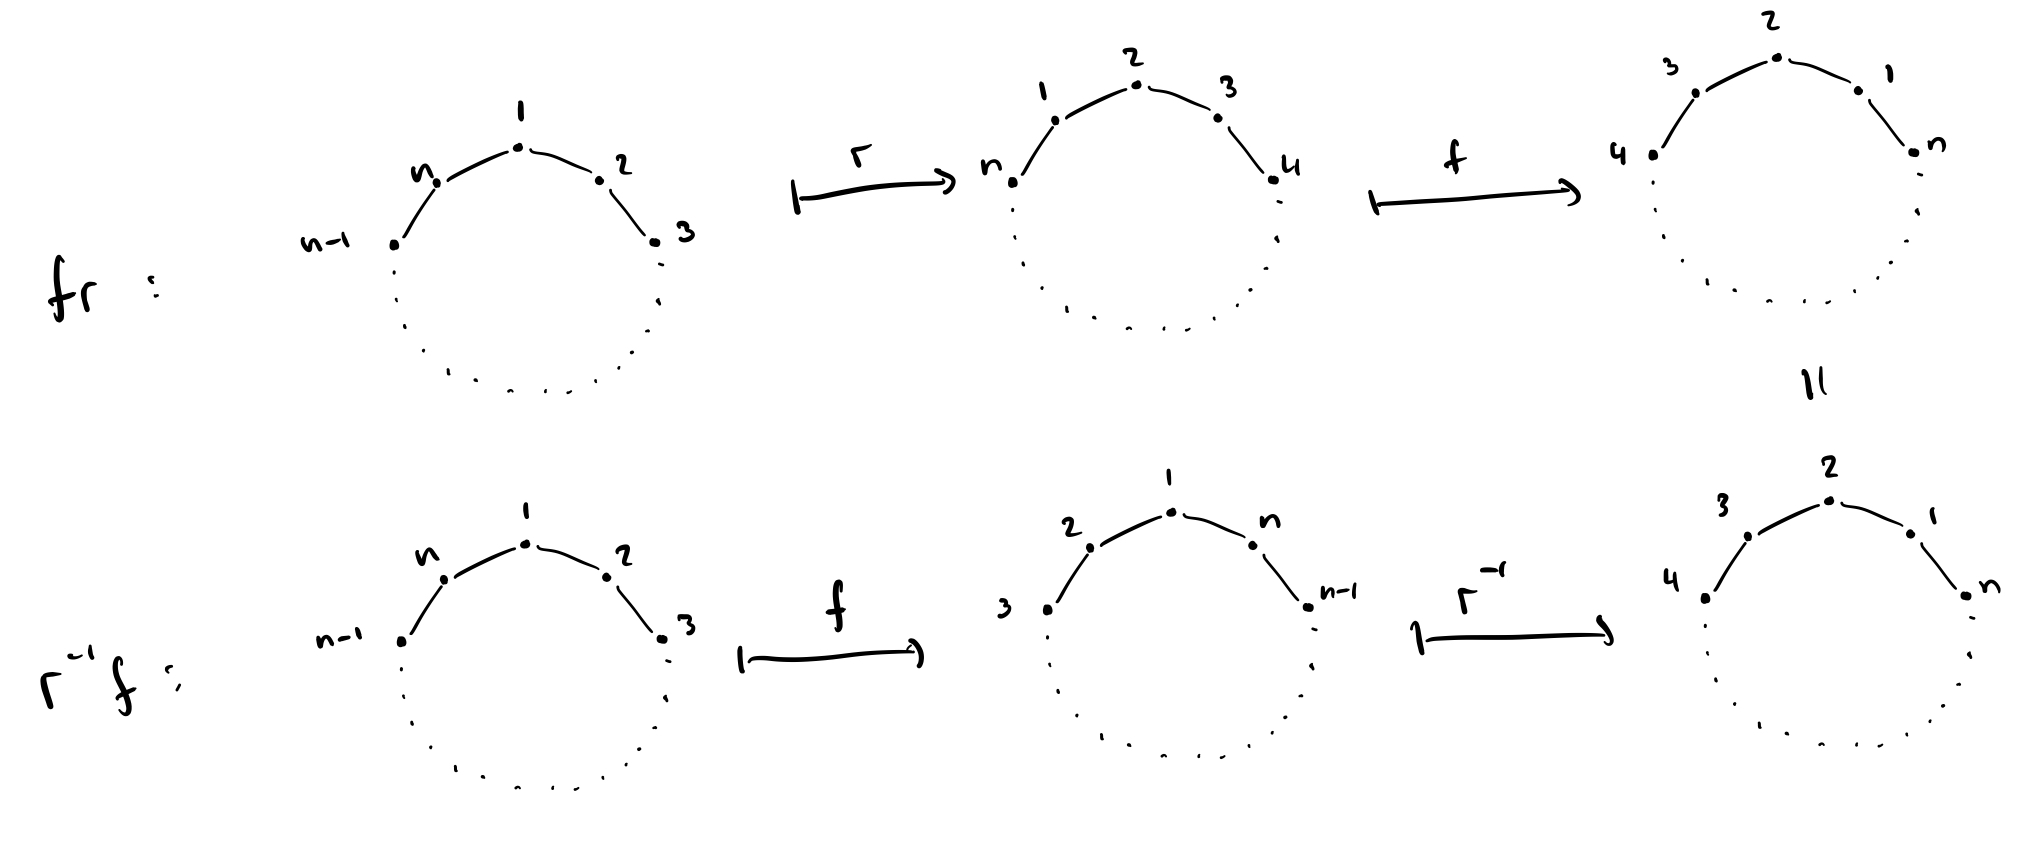
\includegraphics[scale=0.2]{img/fr}
                \caption{Proving $fr = r^{-1}f$}
                \label{fig:fr}
            \end{center}
        \end{figure} \\
        As a final fact, we note that rotations commute within each other.
        We know this intuitively through a geometric line of reasoning, but with symbols we have $r^j r^k = r^{j+k} = r^{k+j} = r^k r^j$.
        \begin{enumerate}[label=(\alph*)]
            \item We now show that if $n$ is odd and $a \in G$ such that $ab = ba$ for all $b \in G$ then $a = e$.
            The proof will come in two parts.
            First a lemma: $fr^j$ ($j \in \{0, 1, 2, ..., n-1 \}$) does not commute in $G$ for $n > 2$.
            We can prove this by finding an element $b \in G$ that does not commute with $fr^j$.
            Take $b = r \in G$, then we have $ab = fr^j r = fr^{j+1}$ and $ba = rfr^j = fr^{-1}r^j = fr^{j-1}$
            But then $ fr^{j+1} = fr^{j-1} $ only for $n \leq 2$.
            So if $a = fr^j$ then $a$ cannot commute if $n > 2$. \parspace
            So we must have $a = r^j$ for some $j$.
            Suppose $j \neq 0$, can $r^j$ commute?
            Take $b = f r^{n-j}$, then $ab = r^j f r^{n-j} = r^j r^j f = r^{2j} f$ and $ba = f r^{n-j} r^j = f$.
            Then $r^{2j} f = f \iff r^{2j} = e$ (right multiply by $f$).
            Then we must have $r^{2j} = r^n$.
            But since $n$ is odd and $j \neq 0$, we have reached a contradiction and must have $j = 0$.
            So for $a$ to commute in $G$, $a$ can only be the identity $r^0$ which commutes by group axioms.
            Therefore, if $n$ is odd the only element that commutes in $G$ is the identity element.
            \item Now we show if $n$ is even that there exists $a \in G$ such that $a \ne e$ and $ab = ba$ for all $b \in G$.
            Pick $a = r^{n/2} \in G$ ($r^{n/2}$ is a member of $G$ because $n$ begin even implies that $n/2$ is an integer).
            Now we show that $r^{n/2}$ commutes.
            Let $b = f^k r^j$ be an arbitrary element of $G$.
            There are two cases.
            Case $k = 0$: we must show $r^{n/2} r^j = r^j r^{n/2} $ which is true because there are only rotations.
            Case $k = 1$: we must show $r^{n/2} f r^j = fr^j r^{n/2}$.
            Beginning with the LHS, $r^{n/2} f r^j = f (r^{-1})^{n/2} r^j = f r^{n- n/2} r^j = fr^{n/2}r^j = f r^j r^{n/2}$ as desired.
            So for an even $n$, the dihedral group has a commuting element that is not the identity.
            \item So now we must find all the commuting elements in $G$ for even $n$.
            First consider the case $n = 2$, then $G = \{ r^0, r^1 \}$ (for $f = r$ by inspection).
            Both elements commute and there are no others to even consider.
            Now let $n$ be an even integer larger than 2.
            From the lemma in part a, we know that a commuting element cannot be of the form $fr^j$ so we need only consider pure rotations $r^j$. \parspace
            We now give a necessary condition for an element to commute in $G$.
            For an element to commute in $G$, it must commute with $f \in G$.
            So we must have $ab = r^j f = fr^j = ba$.
            However, we already know $fr^j = r^{n-j}f$ so we must have $r^j f = r^{n-j}f \iff r^j = r^{n-j}$.
            That is to say, for a rotation $r^j$ to commute it must equal its own inverse.
            There are only two rotations that satisfy equaling their own inverse: $r^0$ and $r^{n/2}$.
            But we already know that both $e, r^{n/2}$ commute so they must be the only elements to commute!
        \end{enumerate}
    }
\end{exercise}

% hw problem 4 -----------------------------------------------------------------

\newpage
\section*{Custom Problem}
    \problem{
        Find the order of the group $Sym(\Q)$ of the (rigid) symmetries of the cube $\Q := [-1,1]^3 \subset \R^3$.
        The task is not to just get the number but to organize all the possible symmetries and build a narrative that gets one to the answer in a rigorous way resting on few, easy to grasp geometric facts.
    }
    \proof{
        To begin, we label the sides of a cube like we would a dice (opposite side sum to seven).
        Figure \ref{fig:dice} shows sides 1, 2, and 3.
        Additionally, we take side 3 to be orthogonal with the z axis and side 1 to be orthogonal with the x axis. \parspace
        Then suppose we were to fix ourselves looking from the positive x axis.
        In the current cube configuration, we would be looking at side 1.
        We note that the number of symmetries of a cube is the same as the number of possible configurations we can see from our vantage point on the positive x axis.
        Because the trnasformation on the cube must be rigid, knowing one side and the initial configuration of the cube allows us to determine the positions of the missing four vertices.
        So all we really need to do is to determine how many configurations we can see from our vantage point on the x axis.
        \begin{figure}[h]
            \begin{center}
                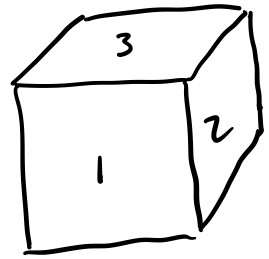
\includegraphics{img/dice}
                \caption{Faces of $\Q$}
                \label{fig:dice}
            \end{center}
        \end{figure} \\
        Let's define two operations: $r$ a counter clockwise rotation by $\pi/4$ about the x axis and $s$ a counter clockwise rotation by $\pi/4$ about the z axis.
        If we were to require that we must view side 1 from our position, there would be four possible symmetries $r^j$ where $j=0,1,2,3$.
        Any remaining symmetries can be obtained by configuring the cube so that we view a different side and the applying the four possible rotations.
        We now give the transformations that bring each side into our field of view.
        \begin{itemize}
            \item side 1: $r^0$
            \item side 2: $s^3$
            \item side 3: $sr$
            \item side 4: $s^3r$
            \item side 5: $s$
            \item side 6: $s^2$
        \end{itemize}
        Then there must be $4*6 = 24$ (four for each side) possible symmetries of the cube.
    }

\end{document}
